% Design of Algorithms (1 week)

\deff{Algorithm}{An algorithm is a well-defined computational procedure with input values and output values.}

In order to be able to compare different algorithms, they are compared in terms of their efficiency. For the \emph{computational time}, the proportionality relationship between the \emph{running time} (number of primitive operations) and the input size $N$ is decisive. A simplified parameter is the order of growth $\Theta$ (e.g. $\Theta(N^2)$ or $\Theta(\log N)$), which describes how the running time scales with the input size $N$. For each algorithm, it is possible to determine what the running time is in the best case (lower bound) and in the worst case (upper bound).

\subsection{Brute Force}

\deff{Brute Force}{Brute force refers to an algorithm that solves the problem exclusively in a linear fashion, which is usually very inefficient.}

The brute force algorithm to sort a vector of integers is the \emph{Selectionsort} algorithm. In this algorithm, a vector $a$ is sorted by checking for each vector element $i$ (outer loop) individually whether there is a smaller element $j$ in the remaining vector (inner loop) and, if so, swapping the smallest element found with the element under consideration. The vector is then sorted from left to right. As the vector is passed through twice, the algorithm with $\Theta(N^2)$ is relatively inefficient.

\begin{center}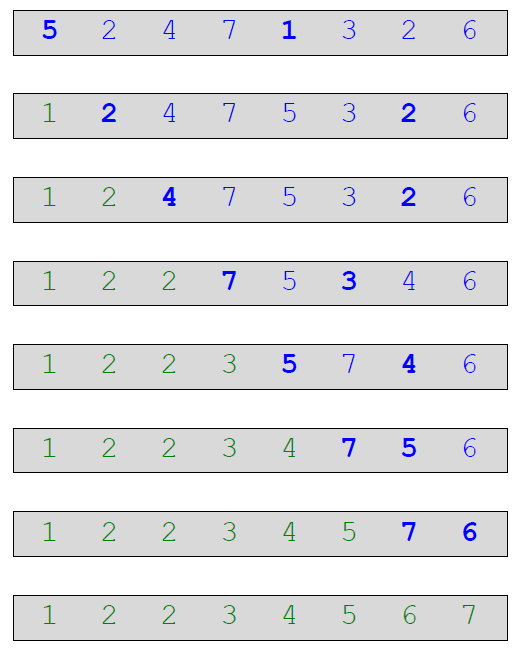
\includegraphics[width=0.45\textwidth]{img/algorithms/BruteForceSelectionsort.png}\end{center}

%\lstinputlisting[language=C++]{src/algorithms/selectionsort.cpp}

\subsection{Divide-and-conquer}

\deff{Divide-and-Conquer}{The divide-and-conquer is a recursive algorithm that consists of dividing the problem into simpler subproblems, solving these individually and finally combining the individual solutions into an overall solution.}
\begin{enumerate}
    \item \textbf{Divide} the problem into a number of smaller subproblems that are smaller instances of the same problem.
    \item \textbf{Conquer} the subproblems by solving them recursively (if the subproblem size is small enough, solve it in a straightforward manner).
    \item \textbf{Combine/Merge} the solutions to the subproblems into the solution for the original problem.
\end{enumerate}

The algorithm is often quite efficient with $\Theta(N\log N)$. A typical example of a divide-and-conquer algorithm is the recursive sorting algorithm \emph{Mergesort}. A vector $a$ is divided into smaller vectors $b$ until the sub-vectors only contain one number. These are then combined to form the sorted vector.

\begin{center}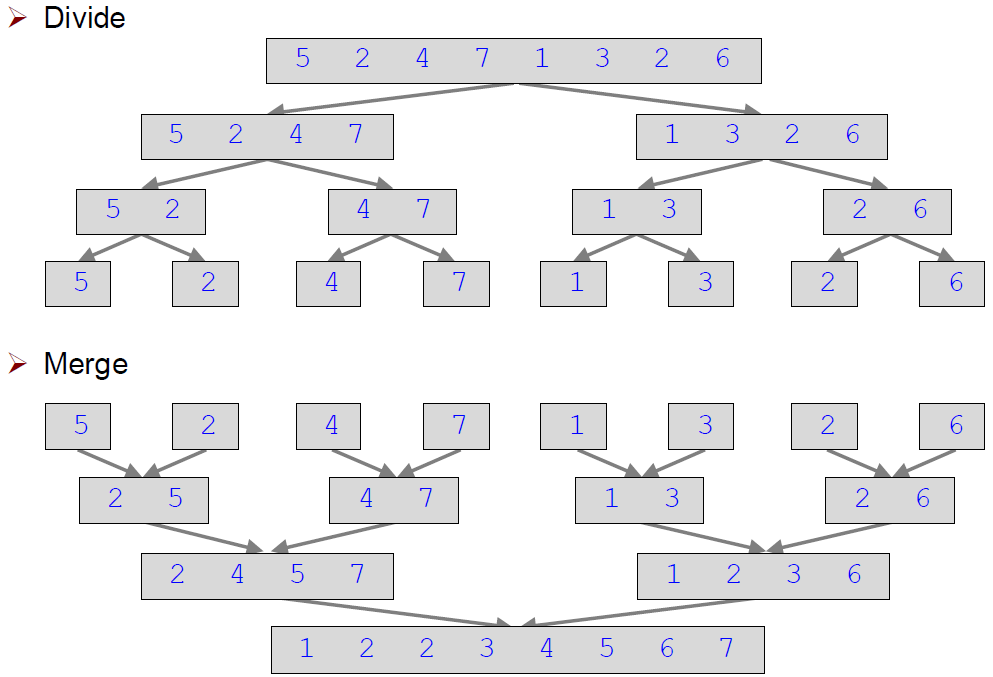
\includegraphics[width=0.85\textwidth]{img/algorithms/DivideConquerMergesort.png}\end{center}

%\lstinputlisting[language=C++]{src/algorithms/mergesort.cpp}

\subsection{Dynamic Programming}

\emph{Dynamic programming} also basically solves problems by combining solutions of subproblems, but here it takes advantage of overlapping subproblems, as individual solutions are used several times. It can be a good technique if the solution to a sub-problem remains good even when integrated into a larger one (e.g. Floyed-Wrashal-algorithm), which is why the algorithm is usually used for optimization problems.

\begin{enumerate}
    \item Solve a subproblem once
    \item Save the result in a table
    \item Look it up if the same subproblem occurs again
\end{enumerate}

A typical problem that can be solved efficiently using dynamic programming is the knapsack problem, in which a knapsack of fixed size $M$ is to be filled with a freely selectable quantity of $N$ different items of different sizes and values. The aim is to maximize the value stored in the knapsack. The running time of this algorithm is with $\Theta(NM)$ clearly smaller than that of the brute force algorithm with $\Theta(2^N)$ for this problem. It is a \emph{bottom-up method} in which the sub-problems are ordered by size. To do this, the Knapsack size is systematically increased and the best solution is determined for each size.

\begin{center}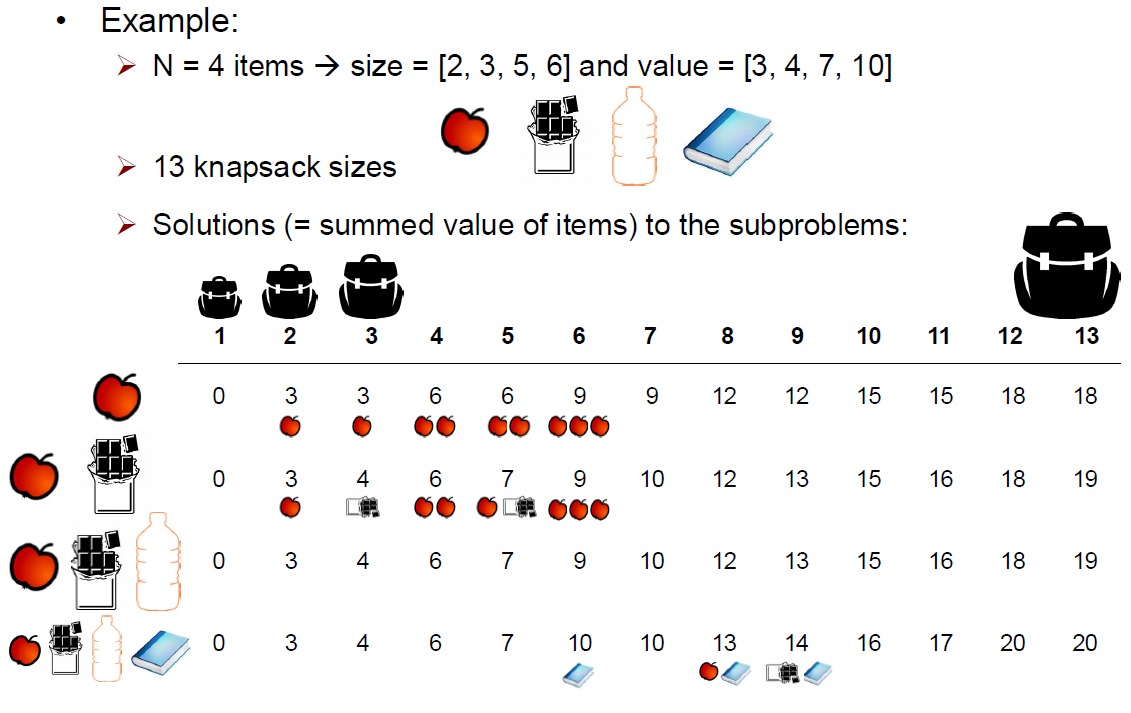
\includegraphics[width=0.85\textwidth]{img/algorithms/DynamicProgrammingKnapsack.png}\end{center}

%\lstinputlisting[language=C++]{src/algorithms/knappsack.cpp}

\subsection{Greedy Algorithm}

A \emph{greedy algorithm} is an approximate algorithm (not necessarily a global optimal solution) that always chooses the option that yields the largest immediate progress towards the goal (= locally optimal) for a sequence of decisions. This class of algorithms is also frequently used for optimization problems or in cheminformatics for MST with Kruskal's algorithm or Prim's algorithm or for Dijkstra's algorithm.

The knapsack problem can also be solved using a greedy algorithm, in which the items with the highest value are packed first, and then the other items are packed in decreasing order of value where $\Theta(N)$ is the running time or $\Theta(N\log N)$, provided that the sorting was done beforehand.

\begin{center}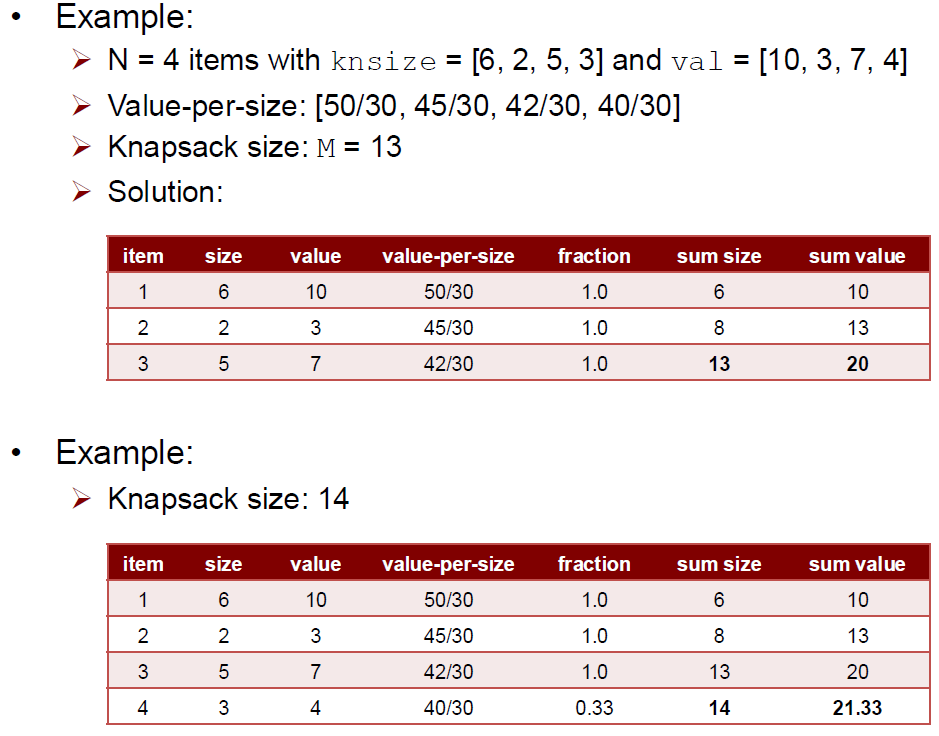
\includegraphics[width=0.85\textwidth]{img/algorithms/GreedyKnapsack.png}\end{center}

%\lstinputlisting[language=C++]{src/algorithms/knappsack.cpp}

\subsection{Backtracking}

\emph{Backtracking} is also an approximate algorithm class in which solution candidates are built and, as soon as it becomes clear that a branch can no longer be the solution, it is canceled and reversed until a solution is possible again. The algorithm is useful for problems where many possibilities first appear, but few survive the constraints or are the “best” solution possibilities (NP-complete problems). The procedure is as follows:

\begin{enumerate}
    \item Rank all possible solutions in the form of a tree $\rightarrow$ solutions are not calculated but classified
    \item Traverse the tree to find a solution which (satisfies a set of given constraints, or is the “best” solution) $\rightarrow$ depth-first tree search
    \item At each node, check whether a subtree of that node can contain a solution $\rightarrow$ if not the case, the subtree can be pruned (skip it)
\end{enumerate}

A typical problem that can be solved with backtracking is the eight queens puzzle, in which eight queens are to be placed on an $8\times 8$ chessboard so that none can capture the others. There are over 4 billion possibilities for this problem, but most of them are eliminated very quickly, which is why backtracking is particularly suitable. If you only use the heuristics of being allowed to place only one queen per row and line, the possibilities are reduced to $40,320$. The running time of the brute force variant would be $\Theta(N!)$ to $\Theta(N^N)$ and that of a backtracking algorithm $\Theta(e^N)$.

\begin{center}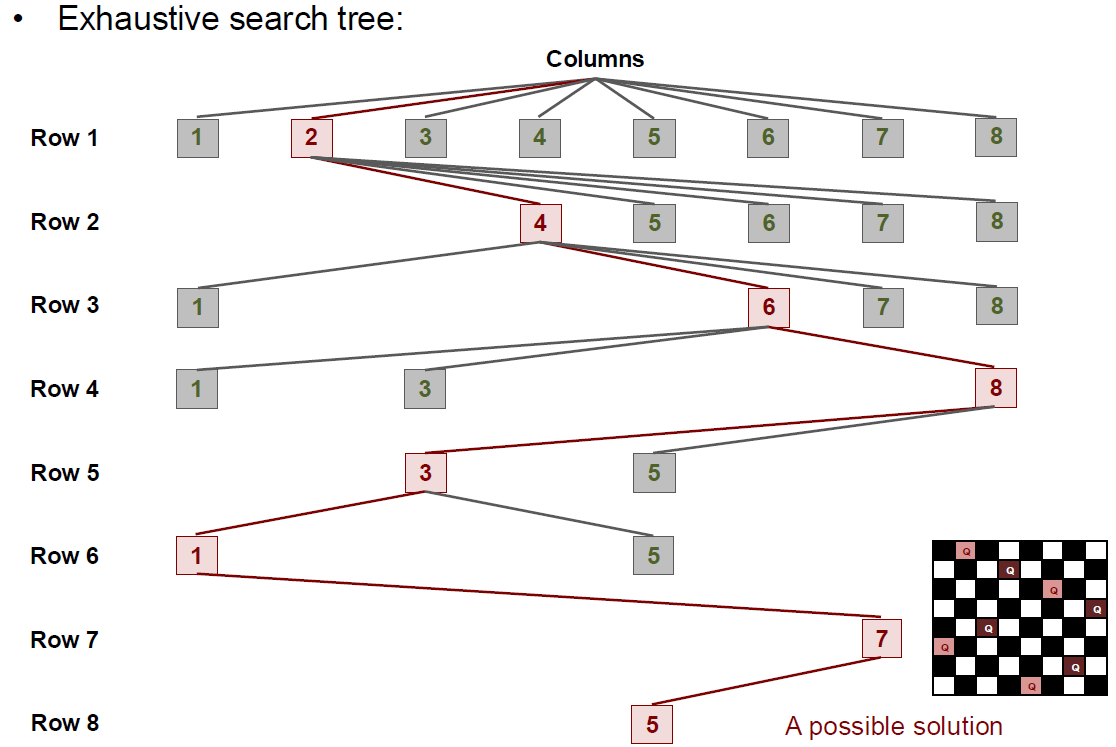
\includegraphics[width=0.85\textwidth]{img/algorithms/BacktrackingEightQueens.png}\end{center}

%\lstinputlisting[language=C++]{src/algorithms/greedy_knappsack.cpp}

\subsection{Local Search}



%\lstinputlisting[language=C++]{src/algorithms/add_queen.cpp}